\hlavicka{PÁTEK 5.1.2007}{č.39}

\section{Bubeníčci 2007 / Revizor 009}

\begin{center}
 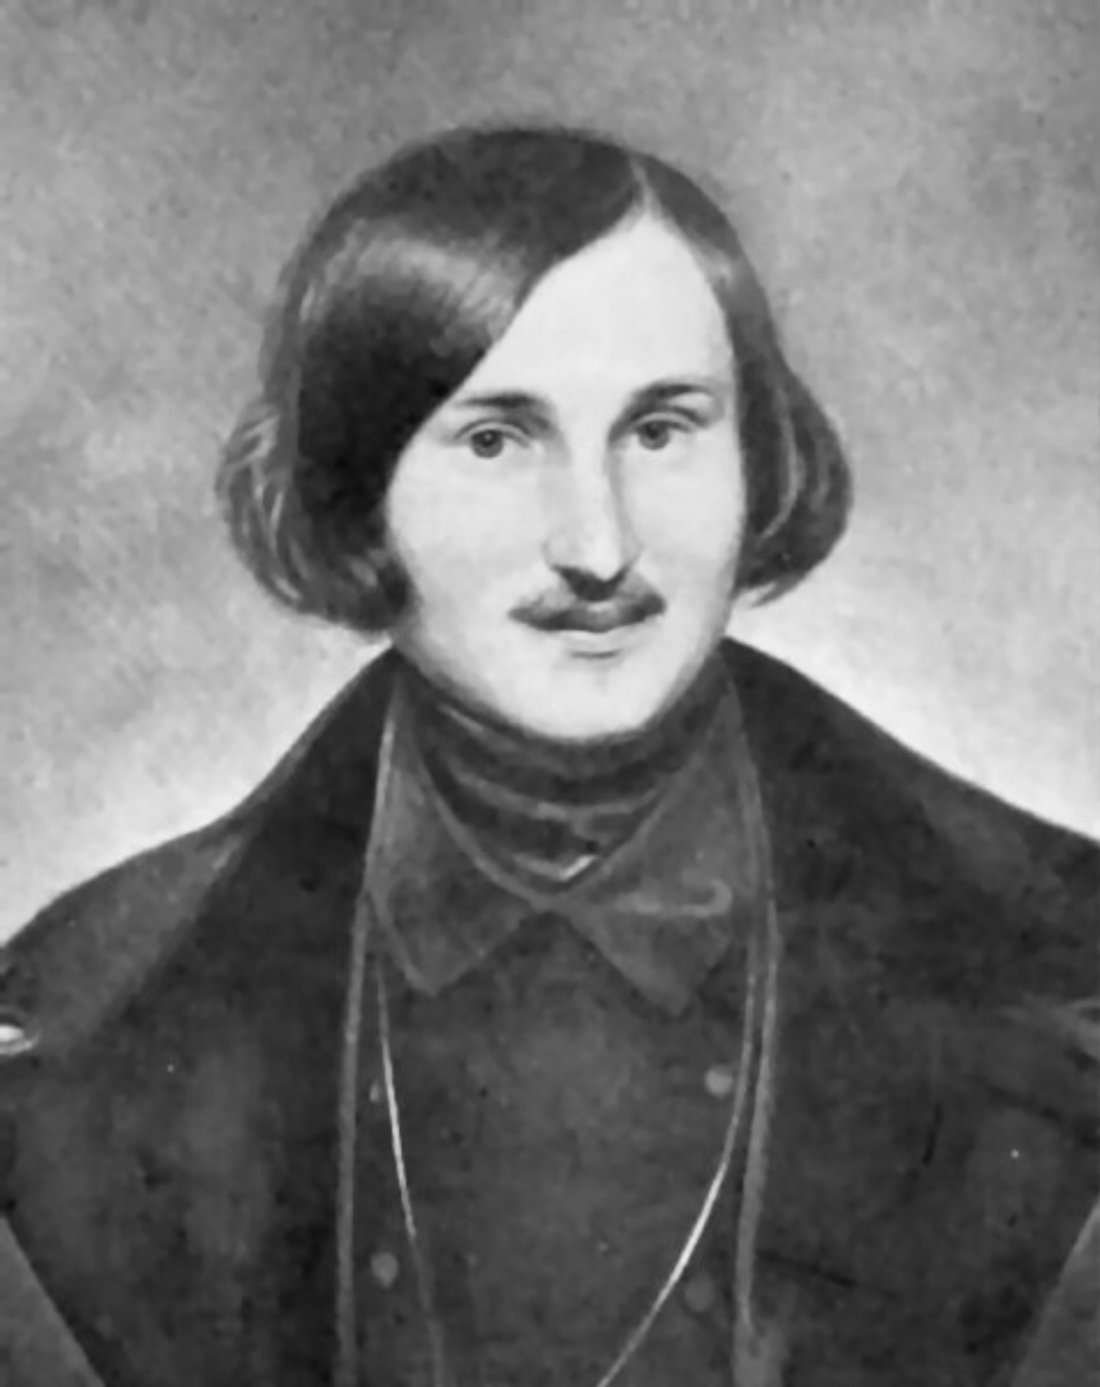
\includegraphics{plavrevue-39/src/gogol.jpg}
 \end{center}

\bigskip

\noindent
Milí přátelé překladatelských Bubeníků! Načínáme tímto měsícem desátý, jubilejní rok našich večerů. A~načínáme jej nadmíru slavnostně. Nestává se často – v dějinách českého divadla tomu bylo ani ne  desetkrát, jak uvidíme –, abychom mohli usednout a v předpremiéře vychutnat nový překlad Gogolova \textit{Revizora}. Usaďte se tedy pohodlně a nechte se jako už mnozí kolébat myšlenkou, že je to o~Nich, protože zrovna Vy byste přece nikdy\ldots

Tentokrát výjimečně neotiskujeme text hry; sama je na rozsah našeho věstníku příliš rozsáhlá a vytrhávání ukázek z kontextu by čtenáře jenom mátlo. Vezměte proto zavděk aspoň malým bedekrem pouti Gogolova \textit{Revizora} českými zeměmi. Cílem tohoto článku není vytvořit separát souvislý, komplexní a zařazený do všech dobových souvislostí; to samo o~sobě by bylo tématem přinejmenším  na diplomovou práci. Rádi bychom však, abyste měli k ruce aspoň stručný přehled, co, kdy a kde se okolo \textit{Revizora} dělo. Však on si to zaslouží, vždyť jde o~jednu z nejhranějších překládaných komedií. Proč, to ovšem přenechme libovolnému divadelnímu programu. \textit{Revizorem} bavily své diváky už celé generace amatérských i profesionálních herců. Autor článku si dokonce vzpomíná na jisté školní představení, kde v rolích Bobčinského a Dobčinského viděl Jiřího X. Doležala a divadelního režiséra, bývalého uměleckého vedoucího ústeckého Činoherního studia Davida Czesaného. Ale vraťme se zpět ke kořenům, podívejme se tedy na začátky českého ,,kamenného`` divadla.

Historicky nejstarší doložený český překlad s nezvykle dlouhým názvem \textit{Revisor aneb Nenadávej na zrcadlo, máš-li hubu křivou!} je z roku 1865.  Přinejmenším unikátní dějiny Prozatímního divadla, vydané loňského roku, uvádějí premiéru \textit{Revisora} dne 21. dubna 1865. Režii měl František Karel Kolár, autorem překladu je \textbf{Václav Huttar} a v roli Chlestakova se objevil v obou reprízách František Ferdinand Šamberk. I~v ostatních rolích se objevily tehdejší hvězdy pražského činoherního divadla – Antonín Pulda, Josef Frankovský a další. Jméno překladatele je pseudonym – pod jménem Václav Huttar se skrývá \textbf{Václav Čeněk Bendl Stránický} (1832-1870), dnes již zapomenutý vlastenecky zaměřený básník, prozaik a překladatel z ruštiny. Kromě \textit{Revizora} přeložil například díla A. S. Puškina – \textit{Evžena Oněgina} a \textit{Bachčisarajskou fontánu}.

Už při letmém pohledu zjistíme, že tento překlad stanovil základní prvky, na které jsme zvyklí až po naše časy. Podtitul dodaný Gogolem do revidované verze se od těch dob nezměnil, pouze se stal mottem, a ani ve jménech postav nenajdeme žádný pokus o~ekvilibristiku s příjmeními, v Gogolových komediích tak typickou. Žádný překladatel, aspoň pokud je nám známo, se nepokusil přeložit některá charakteristická jména analogickými slovními hříčkami. A~tak je (až na drobné variace) Zemljanika stále Zemljanikou, Chlopov Chlopovem, Bobčinský Bobčinským a Dobčinský Dobčinským. Při volném přístupu, který v té době panoval v překladech jmen postav například u~Shakespeara, je to téměř udivující, ale tak se rozhodl už první překladatel a tak to zůstalo.

Už o~pouhé dva roky později se vynořuje další překlad – pod stejným názvem – a to ve svazku věnovaném divadelním ochotníkům. V nakladatelství Mikuláš \& Knapp vyšel roku 1867 sešit s dlouhým titulem \textit{Divadelní ochotník: repertorium pro milovníky soukromých divadel. Nové sbírky svazek 4} obsahující dvě hry vhodné pro ochotnické soubory. Kromě ,,frašky v~jednom jednání \textit{Za živa mrtví manželé}`` v něm najdeme i překlad Gógolova (sic!) \textit{Revisora} podepsaný pouhou šifrou \textbf{J. Š.} Kdo se za ní skrýval, můžeme se pouze dohadovat.

Pokud bychom chtěli sledovat cestu \textit{Revisora} dál, můžeme konstatovat první mimopražskou inscenaci Pavla Švandy ze Semčic v Plzni (1867) a obnovení původní inscenace v Prozatímním divadle v letech 1879-1882 ve stejném překladu a téměř totožném obsazení jako v~roce 1865. Ještě první inscenace v Národním divadle (premiéra 20.10.1891) používá stejný, tedy Huttarův překlad. Stačí však vyjmenovat obsazení premiéry: Chlestakov – Josef Šmaha, hejtmanova dcera – Hana Kvapilová, Bobčinský – Jindřich Mošna, Poštmistr – F. F. Šamberk, Školní inspektor – Eduard Vojan(!). Další inscenace – z roku 1902 v režii Jaroslava Kvapila – už ovšem vychází z nového překladu, který pořídil někdy v té době \textbf{Ignác Hošek} (1852-1919). A~tento překlad, poslední ze ,,staré doby``, vydržel v českých inscenacích až do roku 1920. Časově tedy méně než Huttarův, ovšem důvody, proč zastaral, byly poněkud jiné než generační.

Přišla nová doba. Moderní, zrychlená a sportovní. Prostředí hejtmanů, blahorodích, paruk a dlouhých nadýchaných sukní se stalo najednou archaismem, nicméně hra zůstala aktuální pořád (proč, to si prosím nalistujte někde v onom divadelním programu). Vznikly tedy během krátké doby hned tři překlady. Prvé dva si jenom zrychleně pro úplnost vyjmenujme – jsou podepsané jmény \textbf{Bořivoj Prusík} (1872-1928, překlad je v odborných pramenech datován 1920) a \textbf{Václav König} (překlad 1926).  Úpravu \textbf{Jaroslava Bartoše} (1897-1967) z roku 1930 pro loutková divadla uvádíme jen pro úplnost.

Zastavme se krátce u~dalšího, tedy v pořadí již šestého překladu, a to pro jeho autora. Je jím \textbf{Bohumil Mathesius} (1888-1952), univerzální překladatel z ruštiny, čínštiny i němčiny – a především básník. Dal jazykem svého překladu inscenaci Jiřího Frejky v Národním divadle tak moderní tvar, že se z ní stal vzor všech \textit{Revizorů} na dalších třicet let – a to přes všechny další víry, které se během nich přes české divadlo, společnost i jazyk přehnaly. Ladislav Pešek svého divadelního Chlestakova z roku 1936 ještě zopakoval dvakrát – v letech 1948 a 1958, jen protihráči se mu vyměnili – Zdeňka Štěpánka jako Hejtmana vystřídal Saša Rašilov a později Jan Pivec. Bohumil Mathesius byl ostatně i literárním poradcem české filmové adaptace s~Vlastou Burianem z~roku 1934 – a filmoví historici přičítají právě jemu největší zásluhu na tom, že i přes nutná krácení a zjednodušení se podařilo vytvořit komedii vtipnou a dostatečně gogolovskou.

Další překlad vznikl tedy až po dlouhé době. Byl určen pro inscenaci Jana Kačera v Činoherním klubu roku 1967, tedy v~čase, kdy se ze hry o~hloupých reakčních měšťácích mohla opět stát konkrétní místní a dobová satira. Jeho autorem se stal rovněž znalec ruského prostředí, kultury, vážné hudby a dějin, scénárista a dramaturg \textbf{Zdeněk Mahler} (*1928). Veřejnost ho zná spíš jako filmového scénáristu nebo autora svérázných dokumentárních esejů, překládání bylo jenom jeho jakousi zábavou. Mahlerova verze se ovšem trefila do doby a hry natolik, že se stala její integrální součástí a přežila po českých divadlech celou normalizaci, doby porevoluční a hraje se dodnes. I~nejnovější úprava v Národním divadle vychází z tohoto překladu.

Aby byl seznam českých verzí pokud možno kompletní, zmiňme ještě překlad \textbf{Karla Miloty} (vl. jm. Karel Hroch, 1937-1992), básníka, prozaika, esejisty a překladatele z ruštiny. Ten byl publikován s překladatelovým doslovem v roce 1986 nakladatelstvím Odeon.

\ldots A~dál? Právě připisujeme další položku seznamu. Bude nadepsána pořadovým číslem 9 a jménem \textbf{MILAN DVOŘÁK} (*1949). Přejme tedy i novému překladu dalších třicet nebo čtyřicet úspěšných let na scénách českých divadel. A~je to stejné jako vždycky: do zapadlého městečka v zapadlé ruské gubernii přijde dopis\ldots Řečeno s~klasikem: Chlestakov žil, Chlestakov žije, Chlestakov bude žít.

Příjemný večer s \textit{Revizorem} a úspěšný rok 10 bubenického letopočtu za redakci PlavRevue přeje

\podpis{Jan Smolka}


\pagebreak

\vspace*{24cm}
\noindent{\it Elektronickou verzi Plav Revue naleznete na adrese  \url{http://www.splav.cz}{www.splav.cz}.}











